\chapter{Testdurchführungen}
\label{chap:Testphasen}

Es wurden im Rahmen dieser Arbeit eine grosse Anzahl an Messungen und Testfällen durchgeführt. Die Testkonzepte im digitalen Anhang \ref{AnhangDig} geben detailliert Auskunft über die Testdurchführung. Einige Resultate wurden bereits im vorherigen Kapitel eingebunden. Auf den nachfolgenden Seiten werden die bedeutendsten Resultate wiedergegeben. 

\section{Messinstrumente}

Für die Messungen wurde das Panasonic AMG8834 Eval Kit verwendet. Es bietet den Vorteil, dass sich, dank einem Atmel Mikroprozessor und einer bereits vorhandene Software, die Sensordaten als Rohdaten über USB bzw. \ac{UART} mit dem Programm H-Term auslesen lassen. 
Das erstellte C-Programm ConvertValue\_V2\footnote[12]{im digitalen Anhang bereitgestellt} wandelt die Rohdaten in \ac{CSV}-Files um, damit diese mit Matlab und Python verwendet werden können.

Zudem können die Daten zur Echtzeit über das Bluetooth Modul an die zur Verfügung stehende App übermittelt werden, damit die aktuellen Werte visualisierbar sind.

Zur Vergleich der Messwerte wurde das digitale Thermometer Fluke 52-II und die Wärmebildkamera Fluke TI 125 verwendet. Entsprechende Datenblätter sind im digitalen Anhang \ref{AnhangDig} einsehbar.

\section{Grundlagenmessungen}

Die Grundlagenmessungen geben Auskunft über die Eigenheiten des Messprinzips. Dabei wurde einerseits physikalische Aspekte, welche im vorherigen Kapitel erläutert wurden verifiziert und weitere Erkenntnisse dargelegt. Die nachfolgenden Unterkapitel sind abschnittsweise in Fragestellung, Vorgehen und Resultate gegliedert.

\subsection{Streuung}

\textbf{Fragestellung:} Um eine Person zu detektieren, benötigt es eine Temperaturdifferenz zwischen dem Hintergrund und der Person. Daher stellt sich die Frage wie gross die Streuung des Sensor ist. Diese Streuung gibt die minimale Differenz vor, damit eine Person vom Hintergrund unterschieden werden kann.

\textbf{Vorgehen:} In einem 60-minütigen Messdurchgang bei konstanter Umgebungstemperatur von 22.5°C wurde eine gleichmässig 22.6°C warme Oberfläche ausgemessen. In Abbildung \ref{fig:temperaturverhalten} sind die Thermistorwerte(\textcolor{blue}{blau}) und die 64 Pixelwerte(Werte zwischen \textcolor{red}{rot} \& \textcolor{orange}{orange}) dargestellt.
\begin{figure}[H]
	\centering
	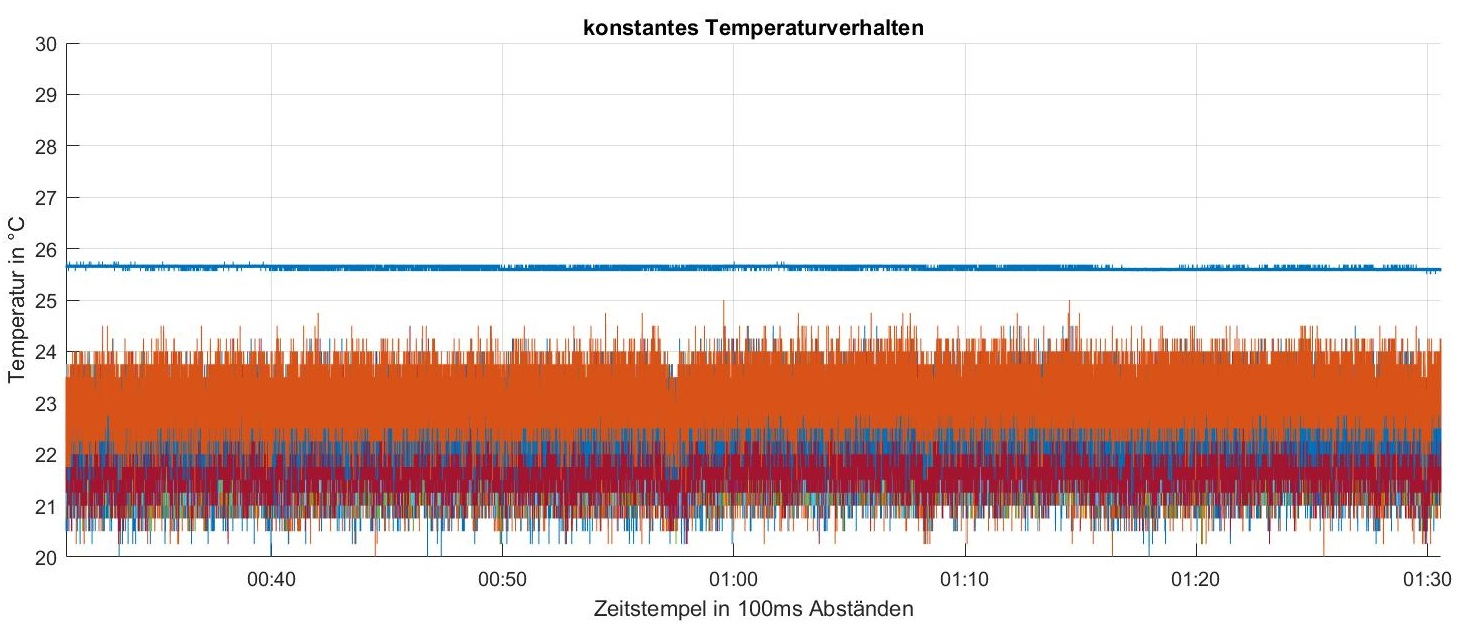
\includegraphics[width=1.0\textwidth]{fig/Temperaturverhalten}
	\caption[konstantes Temperaturverhalten]{konstantes Temperaturverhalten}
	\label{fig:temperaturverhalten}
\end{figure}

\textbf{Ergebnisse:} Es fällt auf, dass  der Thermistorwert(\textcolor{blue}{blau}) entgegen den Erwartungen eine höhere Temperatur (25.5°C anstelle 22.5°C) aufweist. Es wurden mehrere Eval Kits ausgetestet und es konnte kein einheitlicher Offsets\footnote[13]{konstanter Versatz von Effektivwert} eruiert werden. Es ist von Exemplarstreuungen auszugehen. Die Thermistorwerte sind im Allgemeinen um mehrere Grad höher als die effektive Werte. 

Zusätzlich ist in der Abbildung \ref{fig:temperaturverhalten} ersichtlich, dass die Temperaturwerte der einzelnen Pixel nicht auf gleichen Niveau liegen. die Pixelreihe \textcolor{orange}{orange} streut um 23°C, wobei die Pixelreihe \textcolor{red}{rot} deutlich tiefer liegt. Daher kann im Allgemein nicht davon ausgegangen werden, dass die Sensoren bei einheitlicher Oberflächentemperatur, einheitliche Werte liefern. Der Bereich aller 64 Pixel liegt jedoch im Bereich von 3°C. 

Diese Messung bietet eine weitere Erkenntnis im Zusammenhang mit der Streuung. Es wurde in nachfolgender Grafik \ref{fig:Streuung} festgestellt, dass die Sensordaten einer Gaussverteilung\footnote[13]{auch Normalverteilung genant} folgen. Daher wurde die Varianzen\footnote[14]{Abweichung vom Mittelwert} der einzelnen Pixelwerte ausgewertet. Dabei stellte sich heraus, dass die zentralen Pixel tiefere Varianzen aufweisen, als die äusseren Pixel.

Dies könnte in Verbindung mit der konvexen Linse entstehen. Da die Sammellinse an den Rändern mehr Beugungen und Brechungen zulässt. Ein weitere These könnte die grössere Messdistanz aufgrund des \ac{FOV} an den Randpunkte sein. Es muss in jedem Fall mit mehr Abweichungen gerechnet werden, wenn sich Personen am Rande des Messbereichs befinden.

\begin{figure}[H]
	\centering
	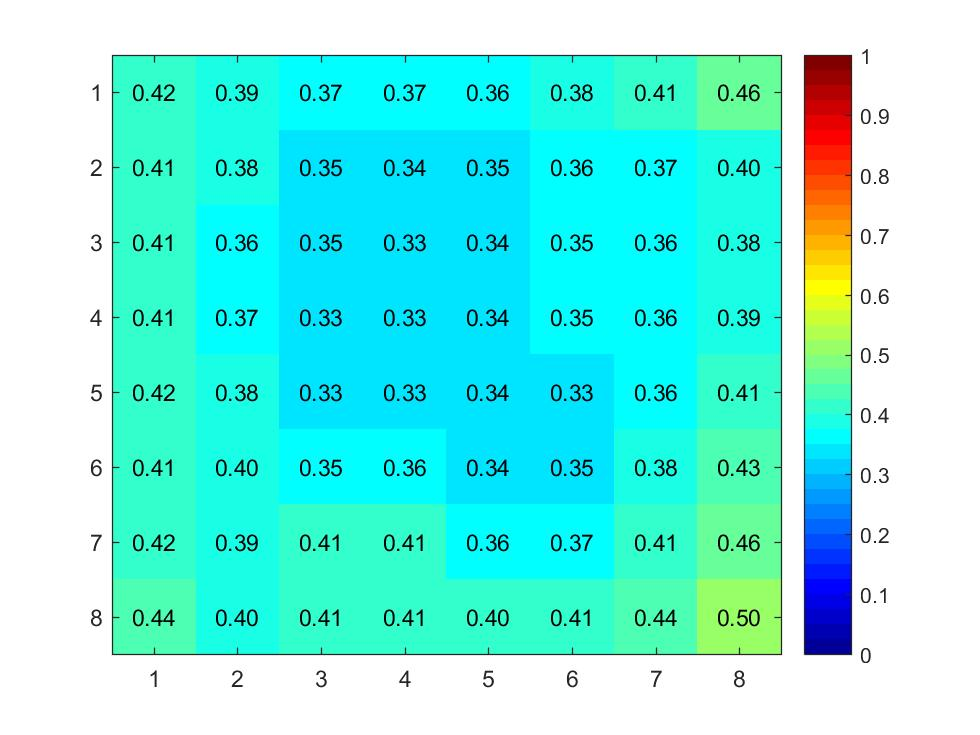
\includegraphics[width=0.5\textwidth]
	{fig/Distanz_140cm_std_.jpg}
	\caption[Streuung der einzelnen Pixel im Vergleich]{Streuung der einzelnen Pixel im Vergleich}
	\label{fig:Streuung}
\end{figure}

\subsection{Einflussfaktor Infrarotstrahlung}

\textbf{Fragestellung:} Der Sensor ist empfindlich auf Infrarotreflexionen und auf die Temperaturen der Messobjekte\footnote{ Unterkapitel siehe \ref{sec:Physik}}. Dabei ist die Sonne eine bedeutende Infrarotstörquelle. Daher wurde im Außenbereich eine Betonoberfläche\footnote[15]{Emissionsgrad 0.92 nach \ref{AnhangE}} ausgemessen, damit Aussagen über die Sonneneinwirkung gemacht werden. 

\textbf{Vorgehen:} In einem kurzen Messaufbau wurde der Sensor abgeschattet von der Sonne platziert. Dabei ist dieser bei einem Abstand von 1m auf eine Betonfläche gerichtet. Die Betonfläche wurde direkt von der Sonne bestrahlt und wird im Verlauf der Messung abgeschattet. Dabei herrschte eine Umgebungstempertur von 25 °C.  


\begin{figure}[H]
	\centering
	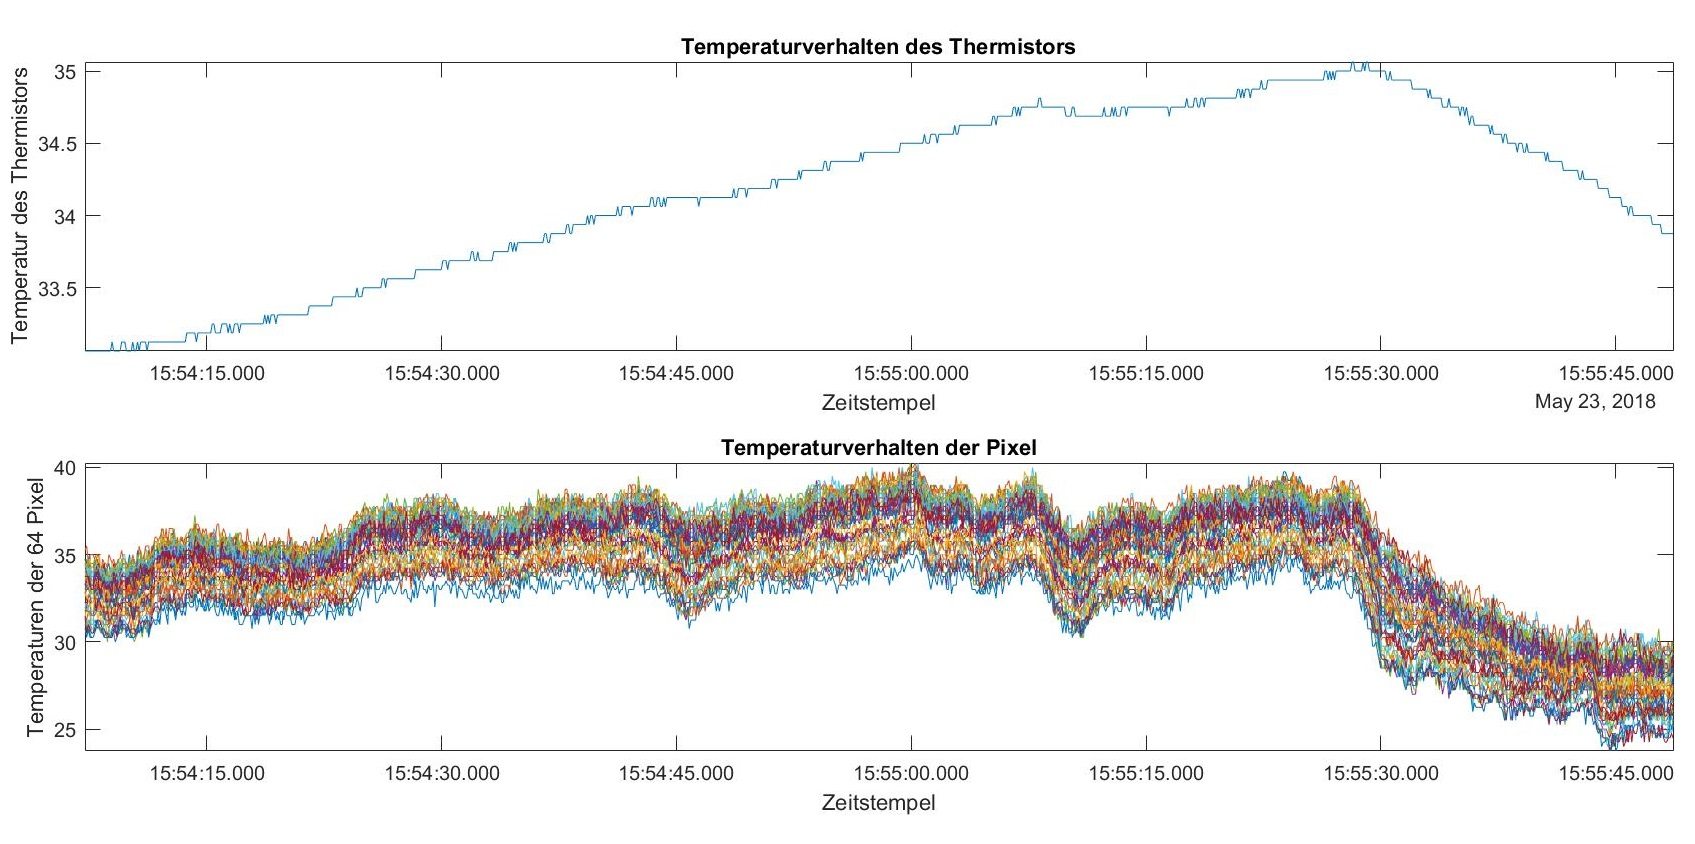
\includegraphics[width=1.0\textwidth]{fig/Temperaturverhalten2}
	\caption{}
	\label{fig:temperaturverhalten2}
\end{figure}

\textbf{Ergebnisse:} In der Abbildung \ref{fig:temperaturverhalten2} sind die Temperatur und Pixelwerte dargestellt. Einerseits ist ersichtlich das bei konstanter Umgebungstemperatur der Thermistorwert weiterhin steigt. Dies hat direkten Einfluss auf die Zunahme der Pixelwerte. Im Aussenbereich ist im Allgemeinen eine grössere Differenz zwischen den Pixeln feststellbar.
Zum Zeitpunkt 15:55:25.000 wird der Messbereich durch eine Holzplatte vom direkten Sonnenlicht abgeschattet. Man erkennt deutlich, dass die Therimstor- und Pixelwerte innerhalb von 15 s bedeutend sinken. Dies hat mit der fehlenden Wärmestrahlung der Sonne zu tun. Daraus kann geschlossen werden, dass Oberflächen, welche direkt von der Sonne bestrahlt stark beeinflusst werden.



\subsection{Einflussfaktor Luftströme}
\textbf{Fragestellung:} Da gerade im Aussenbereich mehr Störquellen für den Sensor vorhanden sind wurden weitere äussere Einflüsse ausgemessen. Dabei stellte sich die Frage, ob auch stärke Luftströme Einfluss auf die Messresultate nehmen.

\textbf{Vorgehen:} Ähnlich wie der vorherige Messaufbau wurde der Sensor und der Messbereich abgeschattet von der Sonne platziert. Dabei ist der Sensor bei einem Abstand von 1m auf eine Betonfläche gerichtet. Dabei herrschte eine Umgebungstemperatur von 25.2°C.  
	
\begin{figure}[H]
	\centering
	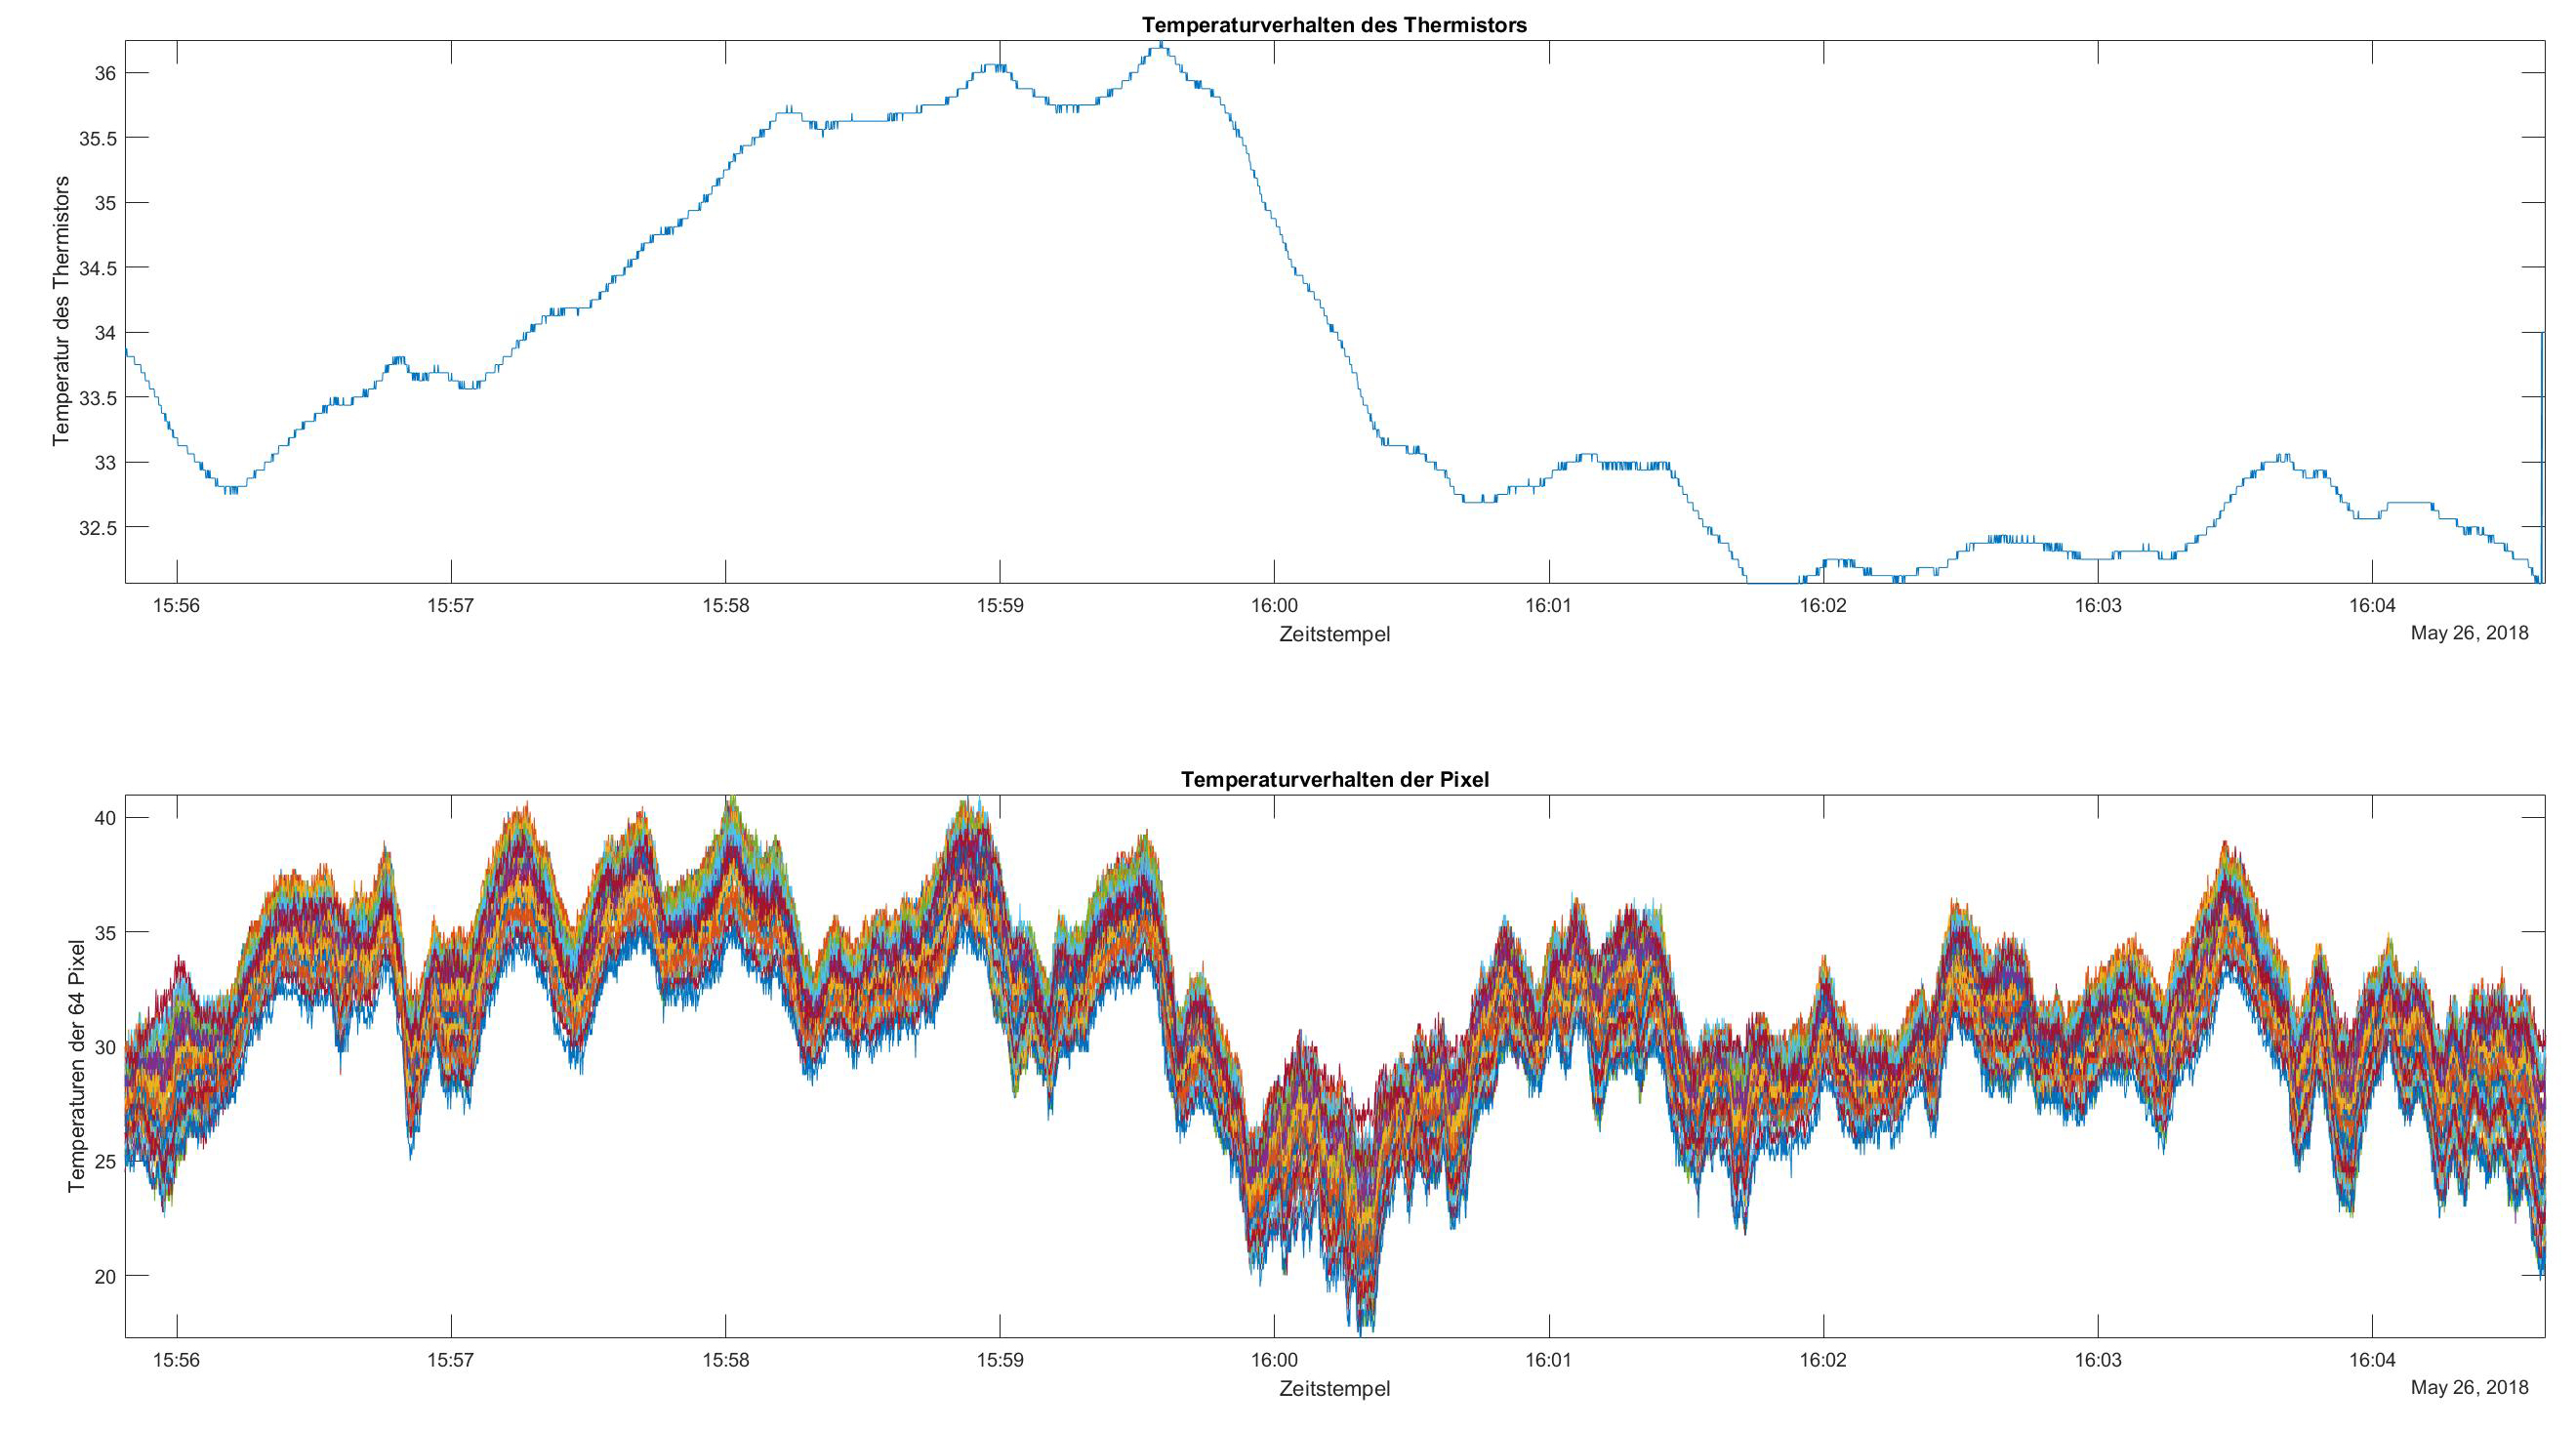
\includegraphics[width=1.0\textwidth]{fig/Temperaturverhaltenwind}
	\caption{}
	\label{fig:temperaturverhaltenwind}
\end{figure}

\textbf{Ergebnisse:} In der Abbildung \ref{fig:temperaturverhaltenwind} sind unregelmäßig Windböen die Ursache für zum Teil starke Abweichungen der Pixelwerte. Die Spannweite der Pixelwerte erstreckt sich zwischen 40 °C bis 18 °C bei, wobei die Temperatur lediglich von 36°C bis 32°C variieren. Somit besitzen Luftströme, wie beispielsweise Wind Einfluss auf die Sensorik. 


\section{Personenmessungen}
Bei der Personenmessungen wurden unterschiedliche Probanden in mehreren Aufzügen ausgemessen und auf dessen Wärmestrahlung analysiert. 

\subsection{Fragestellung} Einerseits soll mit diesen Messungen geklärt werden, wie sich mehrere Personen auf den Messbereichs des Sensors Verhalten und anderseits dienen diese Messdaten gleichzeitig den Datensätzen für die weitere Schritte.

\subsection{Vorgehen}
Es standen insgesamt 6 Probanden zur Verfügung. Die Probanden wurden entsprechend ihrer Grösse und dem Körperumfang in die Kategorien klein [k], mittel [m] und groß [g] unterteilt. Nachfolgende Tabelle gibt über die Masse der Probanden Auskunft. Bei den Werten wurden immer die größten Werte eingetragen.

\begin{table}[H]
\centering
\caption{Masse der Probanden}
\label{my-label}
\begin{tabular}{|
		>{\columncolor[HTML]{C0C0C0}}c |c|c|c|c|}
	\hline
	& \cellcolor[HTML]{C0C0C0}\textbf{Grösse {[}cm{]}} & \cellcolor[HTML]{C0C0C0}{\color[HTML]{333333} \textbf{Breite {[}cm{]}}} & \cellcolor[HTML]{C0C0C0}{\color[HTML]{333333} \textbf{Tiefe {[}cm{]}}} & \cellcolor[HTML]{C0C0C0}\textbf{Kategorie} \\ \hline
	\textbf{Proband 1} & 162                                              & 46                                                                      & 28                                                                     & k                                          \\ \hline
	\textbf{Proband 2} & 166                                              & 52                                                                      & 33                                                                     & k                                          \\ \hline
	\textbf{Proband 3} & 167                                              & 48                                                                      & 25                                                                     & k                                          \\ \hline
	\textbf{Proband 4} & 172                                              & 53                                                                      & 34                                                                     & m                                          \\ \hline
	\textbf{Proband 5} & 175.5                                            & 54                                                                      & 34                                                                     & m                                          \\ \hline
	\textbf{Proband 6} & 185.5                                            & 63.5                                                                    & 42                                                                     & g                                          \\ \hline
\end{tabular}
\end{table}

Für den Messaufbau wurde ein Raster erstellt, welches einerseits den gesamten \ac{FOV} des Sensors abdeckt und anderseits in unterschiedlich grossen Personenaufzügen anwendbar ist. Aus dem Größenvergleich von üblichen Personenaufzügen wurde das nachfolgende Messraster erstellt

\begin{figure}[H]
	\centering
	\includegraphics[width=0.9\textwidth, angle=0]{fig/Messraster_bearbeitet.JPG}
	\caption{Messraster für Personenmessungen}[Messraster für Personenmessungen]
	\label{fig:Messraster}
\end{figure}

In den einzelnen Bildern ist ersichtlich, dass 

\section{Resultate}


\begin{figure}[H]
	\centering
	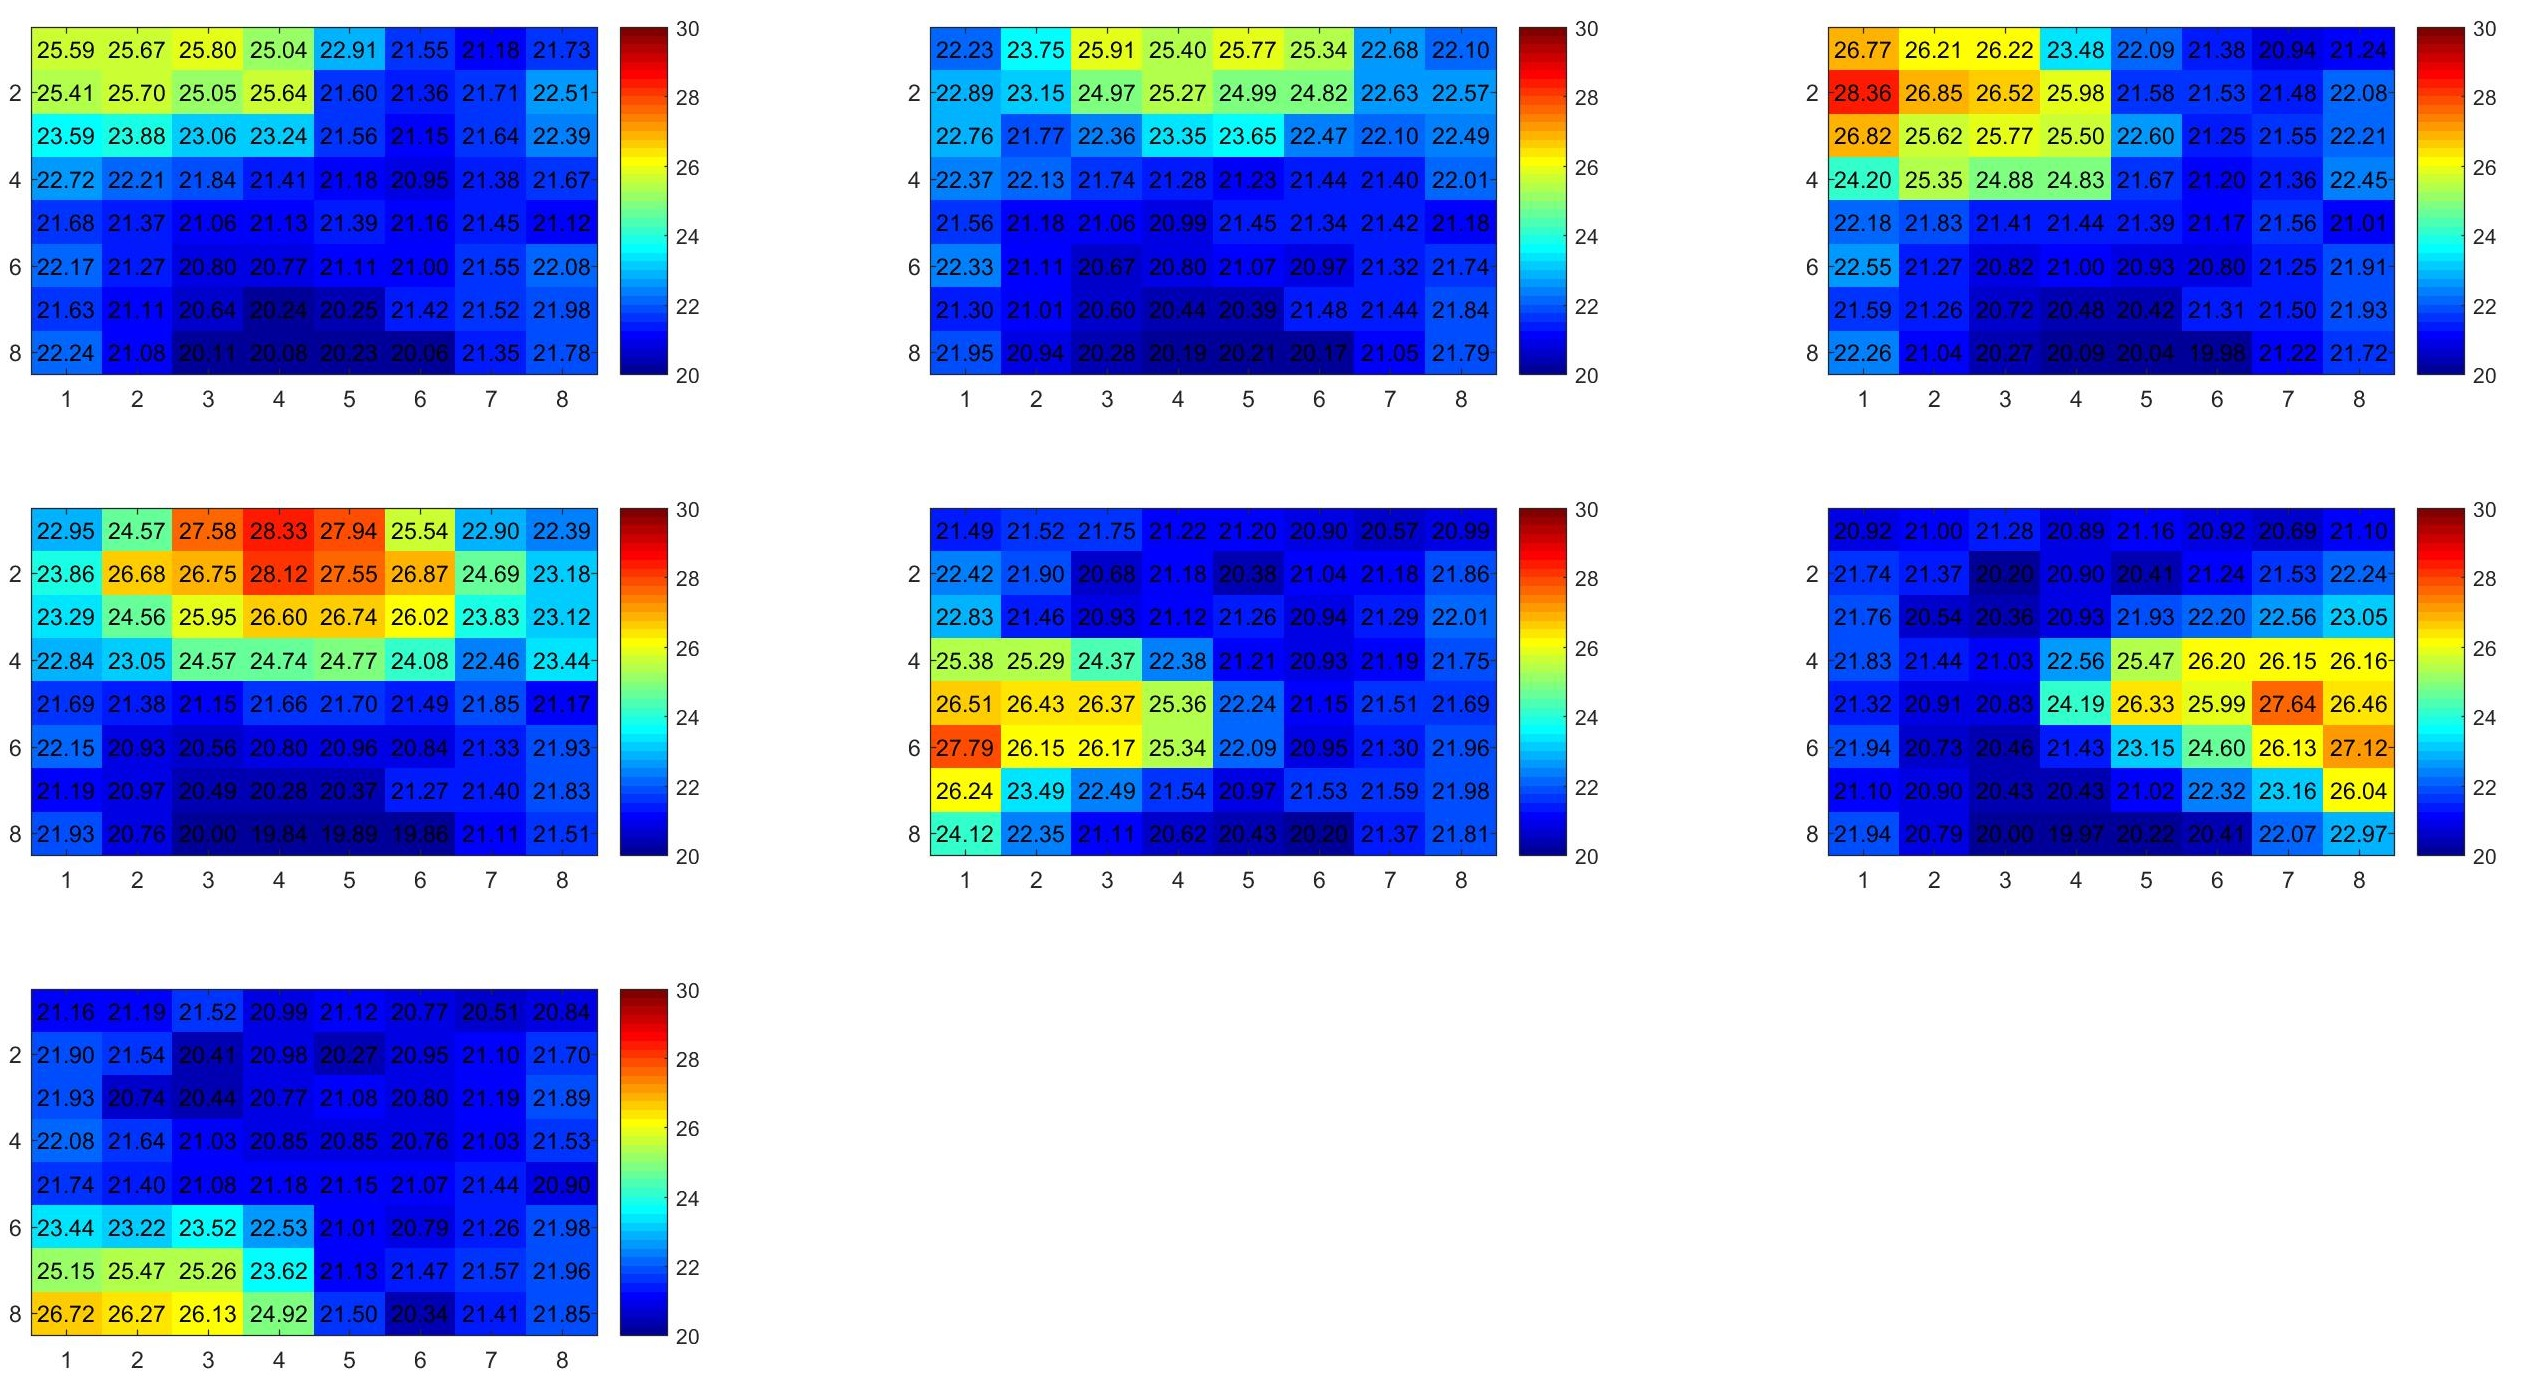
\includegraphics[width=1.0\textwidth]{fig/p1_g_Allpositions_mean}
	\caption[Mittelwerte Messung V1 Kategorie g]{Mittelwerte Messung V1 Kategorie g}
	\label{fig:p1gallpositionsmean}
\end{figure}

In den einzelnen Bildern ist ersichtlich, dass Personen im Zentrum leichter zu erkennen sind. Bei diesen Bilder wird der Kopf, der eine höhe Temperatru aufweist gemessen und daher


\begin{figure}
	\centering
	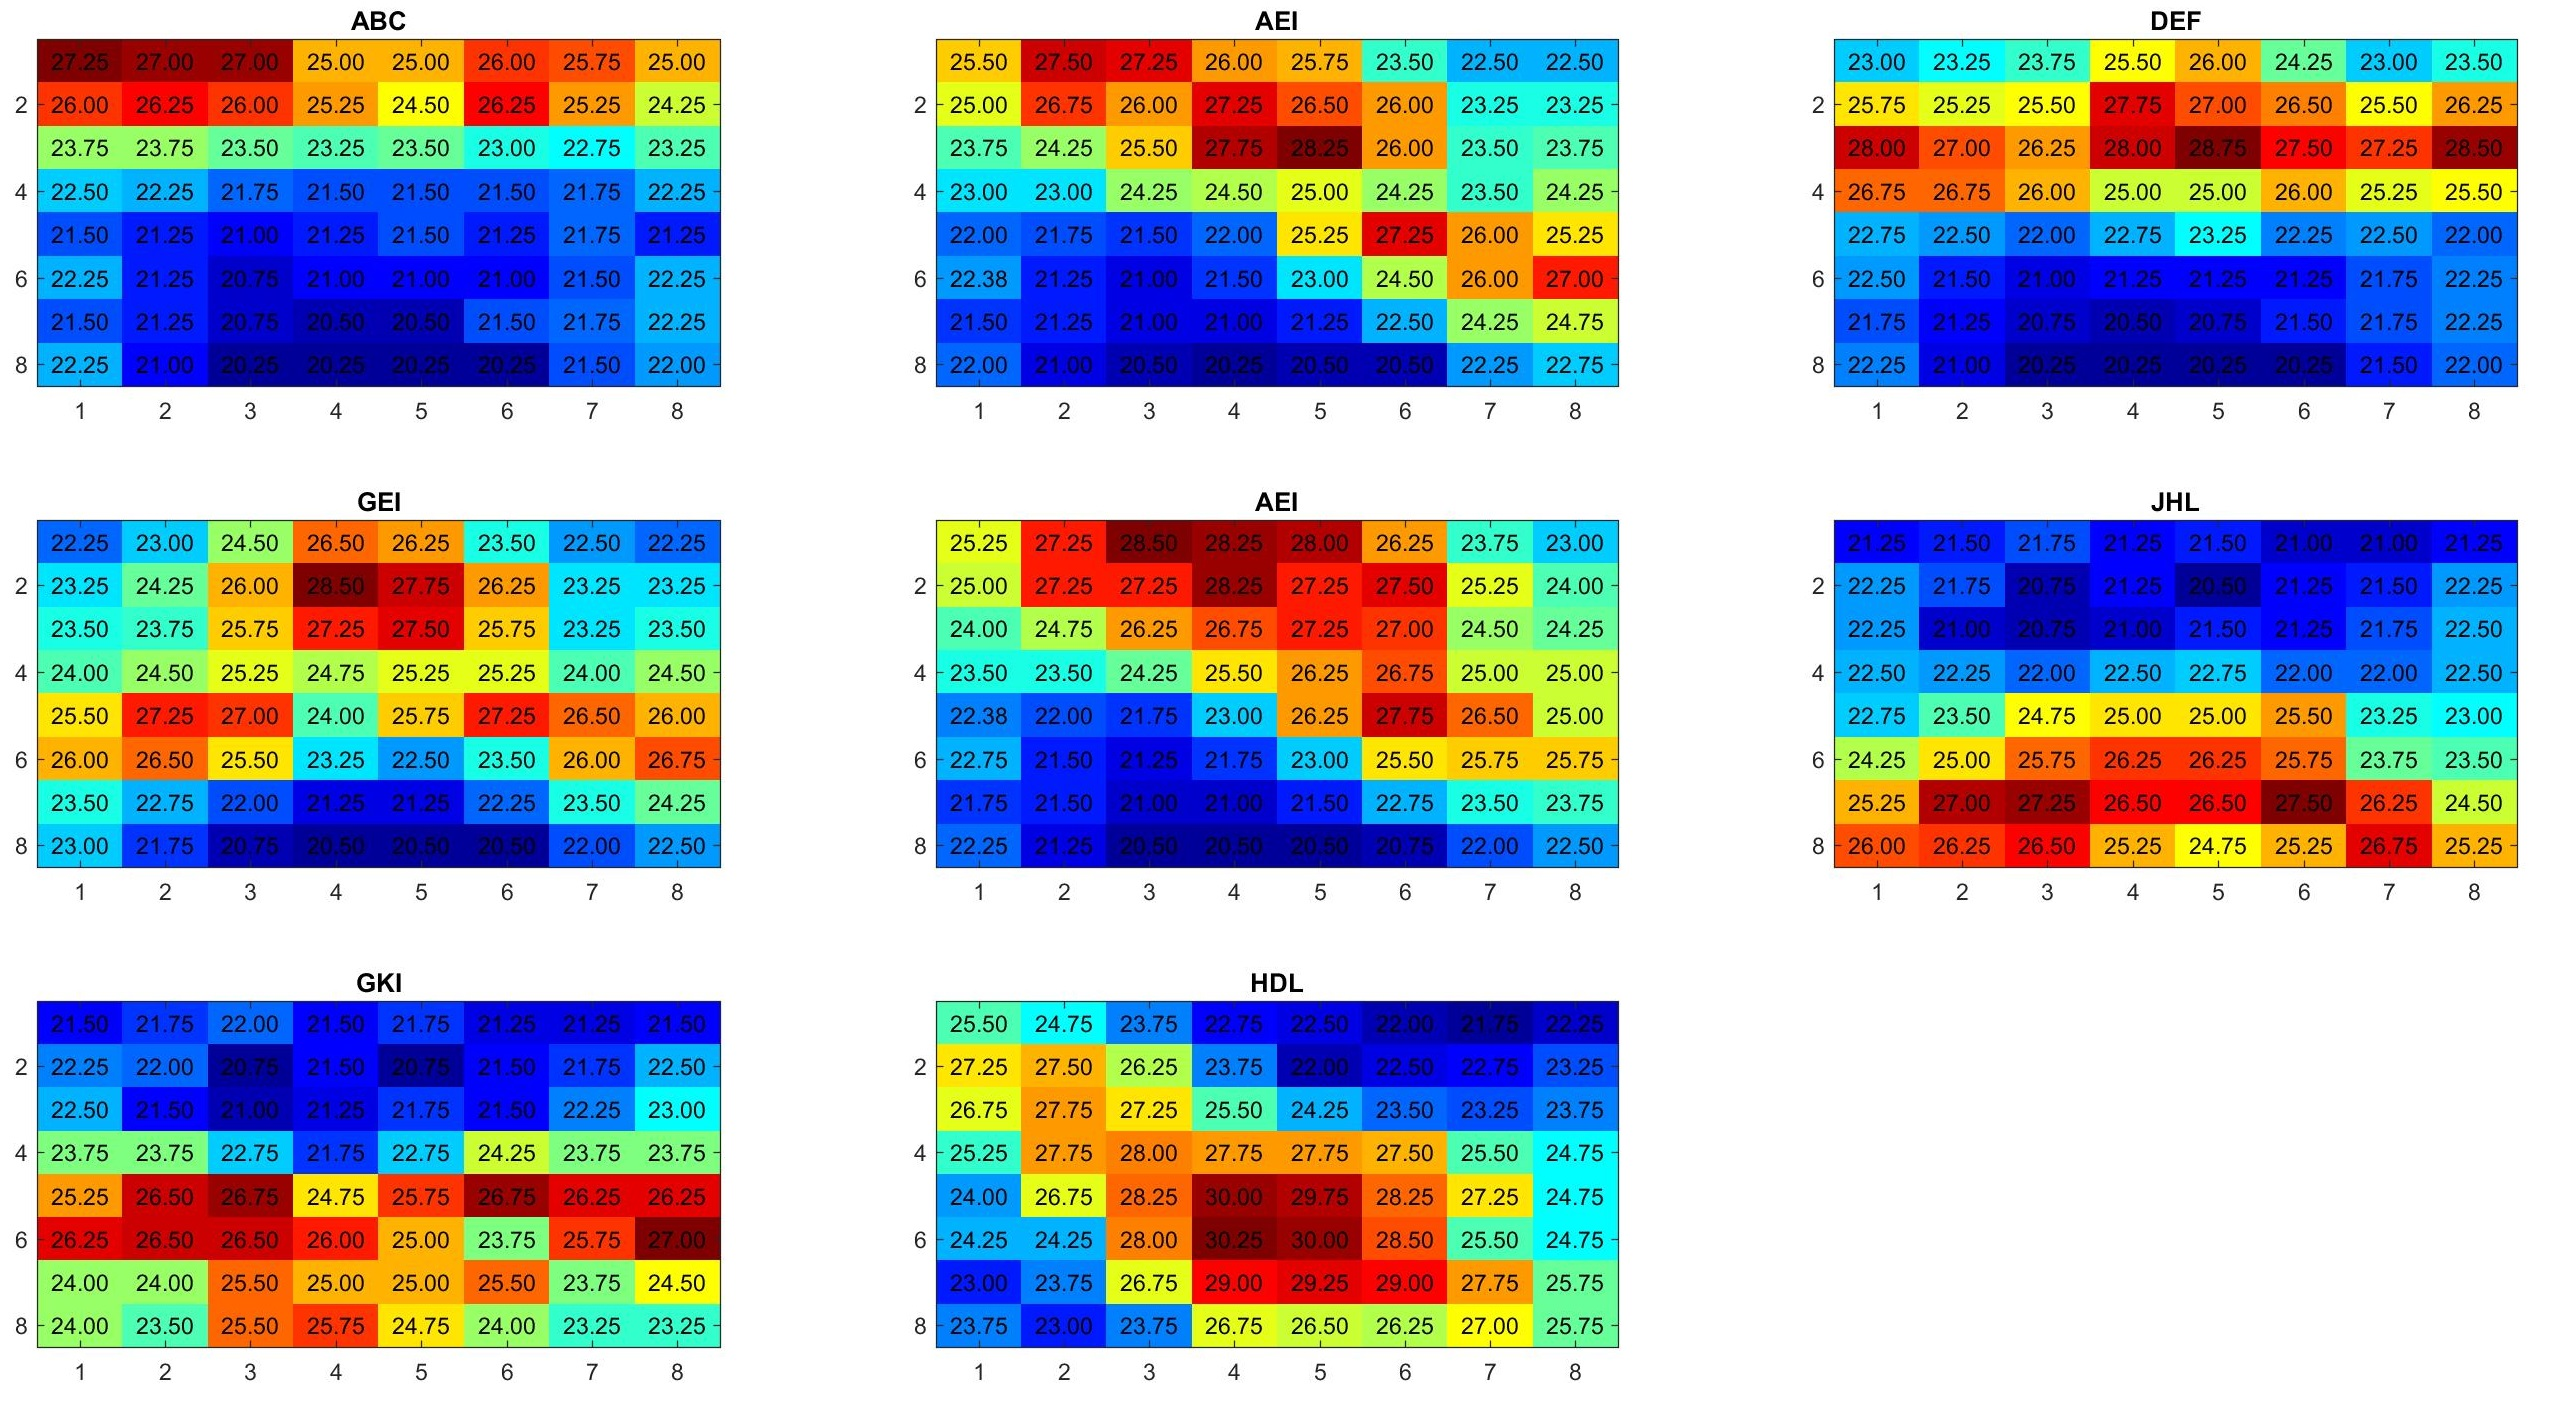
\includegraphics[width=1.0\linewidth]{fig/p3_3x3_allpositons}
	\caption{}
	\label{fig:p33x3allpositons}
\end{figure}







\section{Fazit}
Die Messresultate haben die Ergebnisse aus dem Kapitel \ref{chap:Informationsbeschaffung} bestätigt. Es konnten noch weitere Einlfüsse und Störquellen identifiziert werden. Vor allem im Aussenbereich gibt es grosse Störeinwirkungen, die Einfluss auf die Sensorwerte verursachen . Es liegt nahe, dieses Messprinzip nicht in Aussenbereichen zu verwenden, wenn entsprechende Muster erkannt werden wollen.
 Bei der Personenmessungen liegt die Schwierigkeit bei der Profilbildung von Personen. Da unterschiedliche Umgebungstemperaturen.

